Kalibracija kamere je postopek ugotavljanja notranjih, zunanjih parametrov in koeficientov popačenja. Ena od njihovih uporab je odstranjevanje popačenja. \\
Kalibracija temelji na reševanju osnovnih geometrijskih enačb na podlagi izbranega kalibrirnega objekta. Zaznamo vogale vzorca. Najpogostejši so ChArUco vzorci. Vzorci ChArUco so sestavljeni iz šahovnice in ArUco vzorcev. ArUco markerji imajo hitro zaznavanje, vendar njihova natančnost ni visoka. Šahovnice imajo večjo natančnost, ker je vsak vogal obdan z dvema črnima poljema, vendar mora biti popolnoma viden in ga je težje zaznati. S kombinacijo teh dveh dobimo najboljše od obeh. Z ArUco markerji lahko interpoliramo položaje vogalov šahovnice, kar omogoča delne poglede. Tudi zaradi ArUco markerji ima lahko vsak vogal šahovnice unikaten ID, ki ni odvisen od tega, ali je vzorec obrnjen.

\begin{figure}[h]
    \begin{subfigure}{.5\textwidth}
        \centering
        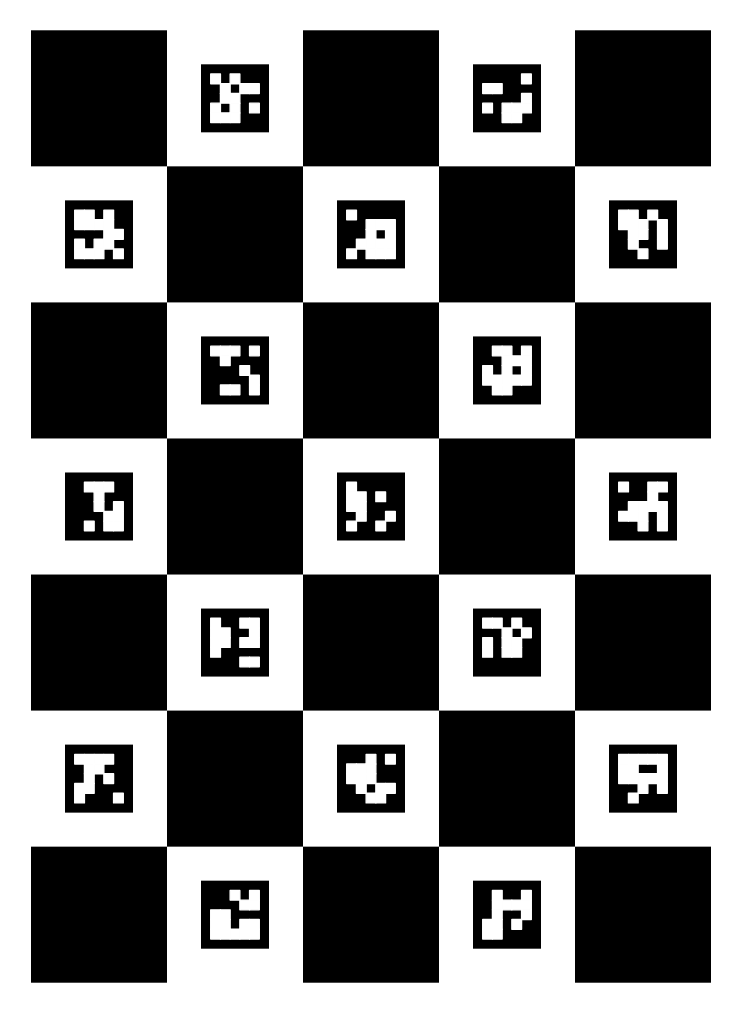
\includegraphics[width=.95\linewidth]{imgs/charuco.png}
        \caption{Primer plošče}
    \end{subfigure}
    \begin{subfigure}{.5\textwidth}
        \centering
        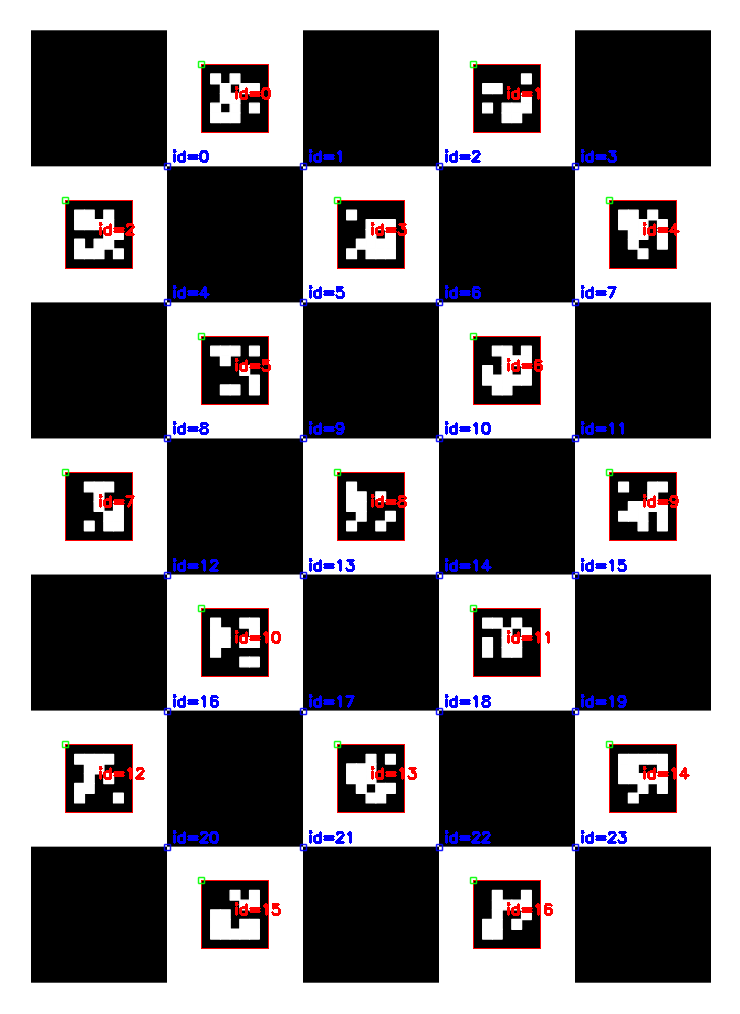
\includegraphics[width=.95\linewidth]{imgs/charucoDetect.png}
        \caption{Plošča z zaznanimi markerji in vrisanimi vogali}
    \end{subfigure}
    \caption{ChArUco plošča}
\end{figure}

\subsection{Zhangova metoda za izračun notranjih parametrov}
V tem pododdelku bomo preučili matematiko v Zhangovi metodi za kalibracija kamere.\cite{zhang}\cite{calibyt}\\

Začnimo s pisanjem enačbe, ki povezuje 3D točko s točko 2D slike. Leva in desna matrika sta notranja in zunanja matrika. Notranja matrika je zapisana nekoliko drugače kot prej, ker tukaj upoštevamo asimetrijo in razmerje stranic(aspect ratio).
\[
    \begin{bmatrix}
    x \\
    y \\
    1 
    \end{bmatrix}
    =
    \begin{bmatrix}
    c   &   cs  &   x_H \\
    0   &   c(1+m)  &   y_H \\
    0   &   0   &   1 
    \end{bmatrix}
    \begin{bmatrix}
    r_{11}   &   r_{12}  &  r_{13}  &   t_1 \\
    r_{21}   &   r_{22}  &  r_{23}  &   t_2 \\
    r_{31}   &   r_{32}  &  r_{33}  &   t_3
    \end{bmatrix}
    \begin{bmatrix}
        X \\
        Y \\
        Z \\
        1
    \end{bmatrix}
\]
S predpostavko, da je $Z=0$ (ko uporabljamo plošče, vse točke na ploščah imajo enako vrednost $Z=0$), lahko odstranimo tretji stolpec zunanja matrike.
\begin{equation}
    \begin{bmatrix}
    x \\
    y \\
    1 
    \end{bmatrix}
    =
    \begin{bmatrix}
    c   &   cs  &   x_H \\
    0   &   c(1+m)  &   y_H \\
    0   &   0   &   1 
    \end{bmatrix}
    \begin{bmatrix}
    r_{11}   &   r_{12}  &   t_1 \\
    r_{21}   &   r_{22}  &   t_2 \\
    r_{31}   &   r_{32}   &   t_3
    \end{bmatrix}
        \begin{bmatrix}
        X \\
        Y \\
        1
    \end{bmatrix}
    \label{simplifiedmappingLong}
\end{equation}
Zelo pomembno je omeniti, da so notranji parametri enaki za vsako sliko (in tako vsako točko na vsaki sliki), medtem ko so zunanji parametri enaki za vsako točko na sliki (spreminjajo se od slike do slike). \\
Transformacijo lahko zapišemo kot 3x3 matriko $H$. Tu je $K$ notranja matrika. Z $H$ lahko zapišemo krajšo obliko \ref{simplifiedmappingLong} za vsako točko $i$, ki je na sliki.
\begin{equation}
H=[\pmb{h_1}, \pmb{h_2}, \pmb{h_3}]=K[\pmb{r_1}, \pmb{r_2}, \pmb{t}]
\label{defH}
\end{equation}
\begin{equation}
    \begin{bmatrix}
        x_i \\
        y_i \\
        1 
    \end{bmatrix}
    =
    H
    \begin{bmatrix}
        X_i \\
        Y_i \\
        1 
    \end{bmatrix}
    \quad
    i=1,...,I
    \label{simMap}
\end{equation}
Od tu naprej, če bi poznali zunanjo matriko, bi lahko samo naredili QR dekompozicijo $H$ in našli naše parametre (Q bi bila zunanja matrika, R bi bila notranja matrika). Vendar ni tako. Najti moramo način z uporabo lastnosti $K$ in zunanje matrike, da izvlečemo $K$ iz $H$. Po tem lahko najdemo zunanje parametre. \\
Začnimo z prepisovanjem enačbe \ref{defH} z inverzijo matrike $K$. Iz te enačbe lahko pridobimo enačbe za $r_1$ in $r_2$.
\begin{gather}
    \begin{bmatrix}
        \pmb{r_1}, \pmb{r_2}, \pmb{t}
    \end{bmatrix}
    =
    K^{-1}
    \begin{bmatrix}
        \pmb{h_1}, \pmb{h_2}, \pmb{h_3}
    \end{bmatrix}   \notag\\
    \notag\\
    \pmb{r_1}=K^{-1}\pmb{h_1} \notag\\
    \pmb{r_2}=K^{-1}\pmb{h_2}
    \label{r1r2}
\end{gather}
Za rotacijske vektorje vemo da so ortogonalni in enotski vektorji. V te enačbe lahko vstavimo enačbe iz \ref{r1r2}. (Opomba: $K^{-T}=(K^{-1})^T$ in $\|\pmb{r_1}\|=\pmb{r_1}^T \pmb{r_1}$)
\begin{gather}
    \pmb{r_1}^T \pmb{r_2}=0 \qquad \Longrightarrow \qquad \pmb{h_1}^TK^{-T}K^{-1}\pmb{h_2}=0    \notag\\
    \|\pmb{r_1}\|=\|\pmb{r_2}\|=1 \qquad \Longrightarrow \qquad \pmb{h_1}^T K^{-T}K^{-1}\pmb{h_1}-\pmb{h_2}^TK^{-T}K^{-1}\pmb{h_2}=0
    \label{hKeqs}
\end{gather}
Definirajmo matriko $B$ in prepišimo \ref{hKeqs}. Ker ima matrika $K$ samo realne vrednosti, je matrika $B$ pozitivno definirana matrika.
\begin{gather}
    B=K^{-T} K^{-1} \label{Bdef} \\
    \pmb{h_1}^T B \pmb{h_2}=0 \notag\\
    \pmb{h_1}^T B \pmb{h_1}-\pmb{h_2}^T B \pmb{h_2}=0
    \label{hBeqs}
\end{gather}
Upoštevajte, da je $B$ matrika, pomnožena z isto transponirano matriko. To matriko lahko najdemo z razcep Choleskega. Z dekompozicijo matrike $B$ bo naš rezultat transponirana inverzna matrika $K$.
\begin{gather}
    chol(B)=A A^T   \notag\\
    A=K^{-T}
    \label{cholesky}
\end{gather}
Torej, če lahko izračunamo $B$, lahko izračunamo $K$. Zapišimo $B$ kot 3x3 simetrično matriko neznank in vektorja $\pmb{b}$, sestavljenega iz teh neznank.
\begin{gather}
    B = \begin{bmatrix}
        b_{11} & b_{12} & b_{13} \\
        b_{12} & b_{22} & b_{23} \\
        b_{13} & b_{23} & b_{33} \\
    \end{bmatrix}   \notag\\\notag\\
    \pmb{b} = [b_{11}, b_{12}, b_{13}, b_{22}, b_{23}, b_{33}]\notag
\end{gather}
Zdaj prepišemo \ref{hBeqs} v obliki sistema $V\pmb{b}=0$(Opomba: $\pmb{v}_{ij}^T \pmb{b}=\pmb{h}_i^T B \pmb{h}_j$) in dobimo:
\begin{gather}
    \pmb{v}_{ij} = \begin{bmatrix}
        h_{i1}h_{j1},   \\
        h_{i1}h_{j2}+h_{i2}h_{j1},  \\
        h_{i3}h_{j1}+h_{i1}h_{j3},  \\
        h_{i2}h_{j2},   \\
        h_{i3}h_{j2}+h_{i2}h_{j3},  \\
        h_{i3}h_{j3}    
    \end{bmatrix}   \notag\\
    \notag\\
    \begin{bmatrix}
        \pmb{v}_{12}^T \\
        \pmb{v}_{11}^T-\pmb{v}_{22}^T
    \end{bmatrix}
    \pmb{b}=0
    \label{vsistem}
\end{gather}

Tu je sistem nedoločen, ker je 2x6 ($\pmb{v}_{ij}$ je 1x6). Uporabimo lahko n slik, ki zložijo enačbe in sistem postane 2nx6. Potrebovali bi 3 ali več slik, da bi bil sistem predoločen, in lahko približne rešitve za sistem tako, da ga minimiziramo z omejitvijo, da je $\|\pmb{b}\|=1$.
\begin{gather}
    \pmb{b}^*=\min_{\pmb{b}}\|V\pmb{b}\|
    \label{bmin}
\end{gather}
S približkom $\pmb{b}$ lahko izračunamo notranjo matriko $K$.

\subsection{Računanje zunanjih parametrov}
Ko najdemo notranje parametre $K$, se lahko vrnemo nazaj in uporabimo \ref{r1r2}. Izračunamo $\pmb{r_3}$ na podlagi tega, da so vsi rotacijski vektorji ortogonalni, in naredimo enačbo za $\pmb{t}$ iz \ref{r1r2}.
\begin{gather}
    \pmb{r_1}=K^{-1}\pmb{h_1} \notag\\
    \pmb{r_2}=K^{-1}\pmb{h_2} \notag\\
    \pmb{r_3}=\pmb{r_1} \times\pmb{r_2} \notag\\
    \pmb{t}=K^{-1}\pmb{h_2} 
    \label{extrinsicequations}
\end{gather}

\subsection{Upoštevanje popačenja}

Kot smo videli v en. \ref{radialdistEq} in \ref{tangentialdistEq}, popačenje ni linearno. Naš cilj je najti te nelinearne parametre popačenja $\pmb{q}$. Lahko ga implementiramo tako, da uvedemo položajni premik (ki je odvisen od položaja $\pmb{x}$ in parametrov popačenja $\pmb{q}$) v $K$.
\[
    K^*=\begin{bmatrix}
        1   &   0   &   \Delta x(\pmb{x, q}) \\
        0   &   1   &   \Delta y(\pmb{x, q}) \\
        0   &   0   &   1
    \end{bmatrix}
    K
\]
Za izračun parametrov popačenja minimiziramo razliko v položaju med točko, kje mora biti in kje je, kjer je za vsako točko na vsaki sliki.
\begin{equation}
    \min_{K, \pmb{q}, R_n, \pmb{t}_n}
    \sum_n  \sum_i
    \|
        \pmb{x}_{ni} - \overset{\wedge}{\pmb{x}}(K, \pmb{q}, R_n, \pmb{t}_n, \pmb{X}_{ni})
    \|^2
    \label{distMinEq}
\end{equation}

\subsection{Povzetek}
Če ponovimo, tukaj so koraki, ki se izvedejo za izračun notranjih, zunanjih in parametrov popačenja.
\begin{enumerate}
    \item Izračunaj $H$ iz več slik s \ref{simMap}
    \item Iz $H$ pridobi $\pmb{v}_{ij}$ in izračunaj $\pmb{b}$ iz več slik \ref{bmin}
    \item Iz $\pmb{b}$ pridobi $\pmb{B}$, izvedi Cholesky razcep, transponiraj in inverziraj ter pridobi notranjo matriko $K$ \ref{cholesky}.
    \item Iz notranje matrike in $H$ izračunaj zunanje parametre \ref{extrinsicequations}
    \item Z minimizacijo aproksimiraj parametre popačenja \ref{distMinEq}
\end{enumerate}